\begin{center}
	\Huge
	Opstilling af differentialligninger
\end{center}

\section*{Sproglig beskrivelse af differentialligning}
\stepcounter{section}

En differentialligning kan også være repræsenteret ved en sproglig beskrivelse, og I skal kunne gå fra sproglig beskrivelse af differentialligning til opstilling af differentialligning. Vi vil gennemgå nogle eksempler. 

\begin{exa}
	Vi har følgende sproglige beskrivelse af en differentialligning: \textit{Væksthastigheden af en population er proportional med størrelsen på populationen}. Vi ønsker at opstille en
	differentialligning på baggrund af denne beskrivelse. Lad os betegne størrelsen af populationen ved $N$. Så vil væksthastigheden være $N'$. Da disse skal være proportionale, må vi have, at 
	\begin{align*}
		N' = k\cdot N,
	\end{align*}
	hvor $k$ er en proportionalitetskonstant. Dette er derfor differentialligningen. Den fuldstændige løsning til denne differentialligning er som bekendt givet ved
	\begin{align*}
		N(x) = ce^{kx}.
	\end{align*}
\end{exa}
\begin{exa}
	Newtons afkølingslov lyder: \textit{Den hastighed hvorved en genstands temperatur aftager er propotional med forskellen mellem genstandens temperatur og omgivelsernes temperatur.} Lad os betegne
	genstandens temperatur med $T$ og omgivelsernes temperatur med $T_{\textnormal{omg}}$. Forskellen på temperaturen og omgivelserne er dermed $T-T_{\textnormal{omg}}$. Dette skal være proportionalt 
	med hastigheden hvorved temperaturen aftager, som er $T'$. Dermed fås differentialligningen
	\begin{align*}
		T' = -k(T-T_{\textnormal{omg}}) = -kT + kT_{\textnormal{omg}}.
	\end{align*}
	Denne differentialligning har som bekendt den fuldstændige løsning
	\begin{align*}
		T(x) = T_{\textnormal{omg}} +ce^{-kx}
	\end{align*}
\end{exa}

\section*{Opgave 1}
\begin{enumerate}[label=\roman*)]
	\item I en begrænset periode oplyses det, at væksthastigheden for en bestemt type bakterie er proportional med koncentrationen af bakterier. Proportionalitetskonstanten er 0.16. Opstil en 
	differentialligning, der beskriver bakterievæksten og brug denne til at bestemme en model for bakteriekoncentrationen. 
	\item Vi opløser salt i vand. Vi opløser i alt 7kg salt ned i en stor beholder med vand. Det oplyses, at hastigheden hvorved saltet opløses er proportional med den mængde salt, der endnu ikke er 
	opløst. Proportionalitetskonstanten er 0.05. Opstil en differentialligningsmodel, der beskriver opløsningen af salt i vand og bestem en fuldstændig løsning til denne differentialligning. 
	\item En cylindrisk beholder har et hul i siden af bunden. Til at starte med er den fyldt med vand. Den hastighed hvormed højden af vandet i beholderen aftager er proportional med kvadratroden af 
	højden. Opstil en differentialligning, der beskriver denne situation.
	\item Størrelsen på befolkningen i en bestemt by beskriver vi med $n$. Bæreevnen (det maksimale antal mennesker) er givet ved $M = 1.2$ mio. Det oplyses, at væksten af befolkningen er proportional 
	med produktet af størrelsen på befolkningen og forskellen mellem befolkningsstørrelsen og bæreevnen. Proportionalitetskonstanten er 1.05. Opstil en differentialligning, der beskriver situationen
\end{enumerate}

\section*{Opgave 2}

I en model for væksten af en bestemt fisk betegner $l(t)$ længden af fisken i cm til tiden $t$ målt i uger. Den hastighed, hvormed $l(t)$ vokser er proportional med fiskens længde og omvendt proportional med $(1+t)^2.$

\begin{enumerate}[label=\roman*)]
	\item Opstil en differentialligning, der beskriver fiskens vækst. 
	\item Løs differentialligningen, når proportionalitetskonstanten er 1.2 og $l(0) = 5$. (Løs med Maple og dsolve)
	\item Hvor lang er fisken efter 4 uger ifølge modellen?
	\item Hvor lang bliver fisken maksimalt?
\end{enumerate}



\section*{Opgave 3}
Følgende er tidligere eksamensopgaver uden hjælpemidler
\begin{center}
	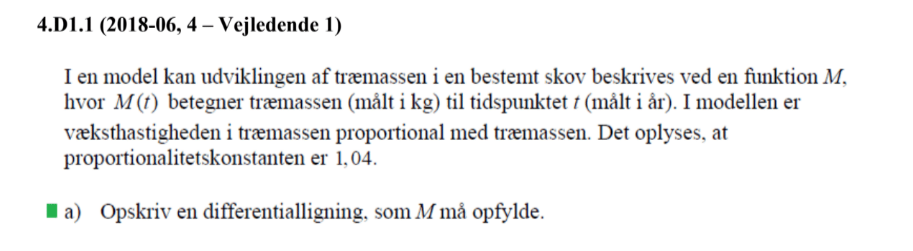
\includegraphics[width=0.7\textwidth]{Billeder/sprogligdiff1.jpg}
	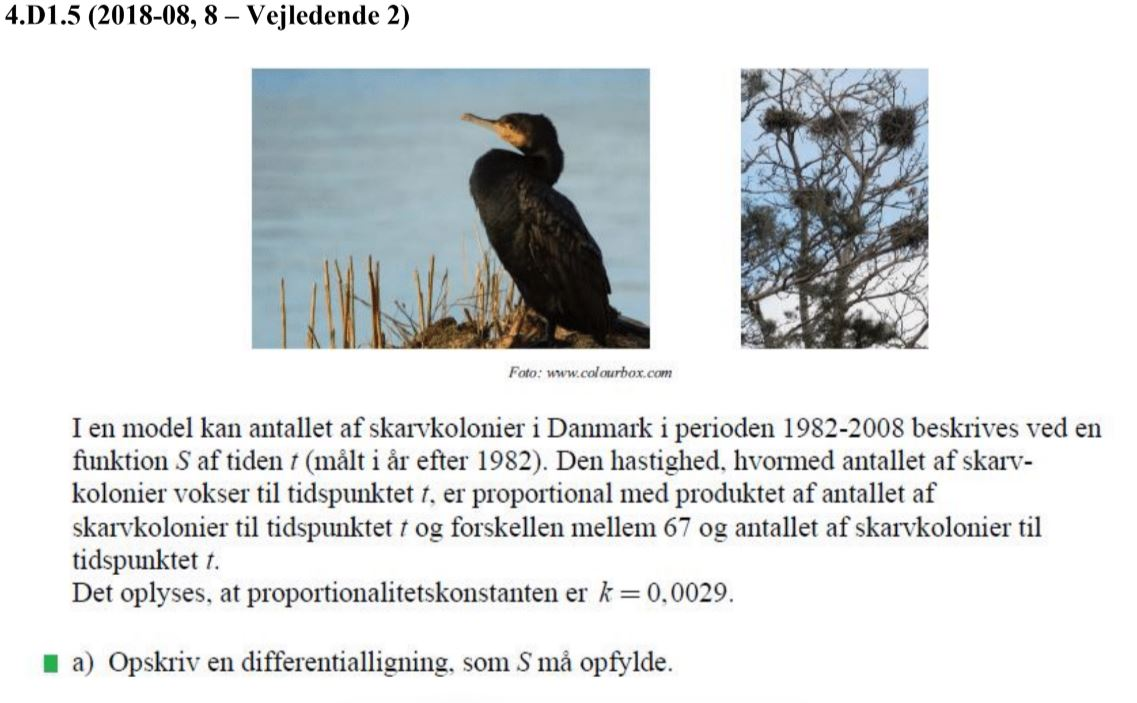
\includegraphics[width=0.7\textwidth]{Billeder/sprogligdiff2.jpg}
	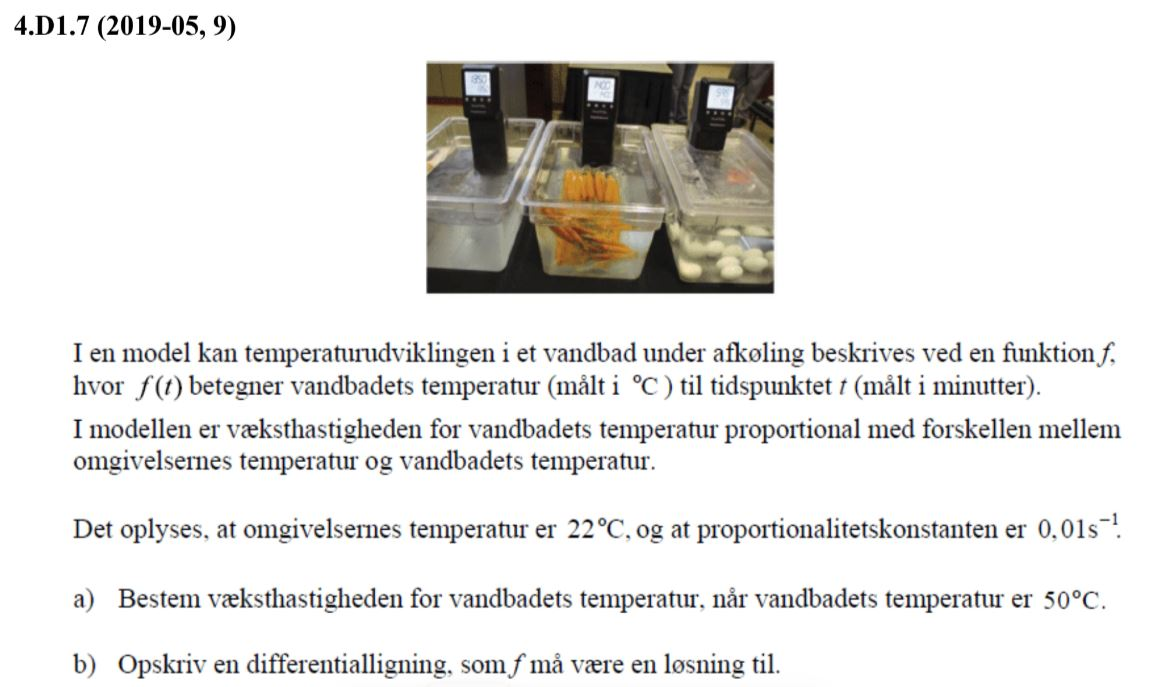
\includegraphics[width=0.7\textwidth]{Billeder/sprogligdiff3.jpg}
\end{center}